\documentclass[aps,pra,notitlepage,amsmath,amssymb,letterpaper,12pt]{revtex4-1}
\usepackage{amsthm}
\usepackage{graphicx}
\graphicspath{{./CW1LaTeXimages/}}
 
\newenvironment{problem}[2][Problem]{\begin{trivlist}
\item[\hskip \labelsep {\bfseries #1}\hskip \labelsep {\bfseries #2.}]}{\end{trivlist}}
\newenvironment{solution}{\begin{proof}[Solution]}{\end{proof}}
 
% --------------------------------------------------------------
%                   Document Begins Here
% --------------------------------------------------------------
 
\begin{document}
 
\title{Homework 1: Remarks on Derivatives}
\author{Alexis \surname{Ford}}
\author{Nengyin (Helen) \surname{Zhu}}
\affiliation{CS 510 -- Computing for Scientists}
\date{\today}

\begin{abstract}
	This paper will give an overview of the derivative, namely, the definition of the derivative of a function, as well as what it means to take the derivative of a function. 
\end{abstract}

\maketitle

\section{Definition}
The derivative of a function $f(x)$, denoted $f'(x)$, is defined as
\begin{equation}
f'(x)=\lim_{h\rightarrow0}\frac{f(x+h)-f(x)}{h}.
\end{equation}
In words, the derivative is the instantaneous rate of change of a function $f(x)$ at $x$, but let us take a more intuitive look. Notice that $\frac{f(x+h)-f(x)}{h}$ bears a strong resemblnce to the formula used to find the slope, $m$, of a line defined by two points, $(x, y)$ and $(x_1,y_1)$:
\begin{equation}
m=\frac{y_1-y}{x_1-x}.
\end{equation}
If we say $h=x_1-x$, and $f(x)$ is the function such that $f(x)=y$ and $f(x_1)=y_1$, we need only note that $h=x_1-x\Rightarrow x_1=x+h$ before the two fractions become identical. Thus, what the derivative is really doing, is finding a slope. 

It is easy enough to find a slope given two points, $a$ and $b$, and we can even estimate the slope of a nonlinear function at a particular point $x$ by creating a secant line using points around our point of interest. The derivative, however, is far more clever than that. By takig the limit as the distance between $a$ and $b$ approaches $0$, we can get the exact, instantaneous rate of change at our point $x$. That is, we get the slope of the line tangent to $f(x)$ at $x$.

\section{An Illustration}
Let us take a look at some pictures to get a better idea of what exactly is going on. Consider the function $f(x)=\frac{1}{10}(x^4-10x^2+9)$, and say we want to find the slope of this function at $x=2$. Let us start by looking at an approximation of the slope using a secant line through the points $(1,0)$ and $(3,0)$.

\begin{figure}[h!] 
  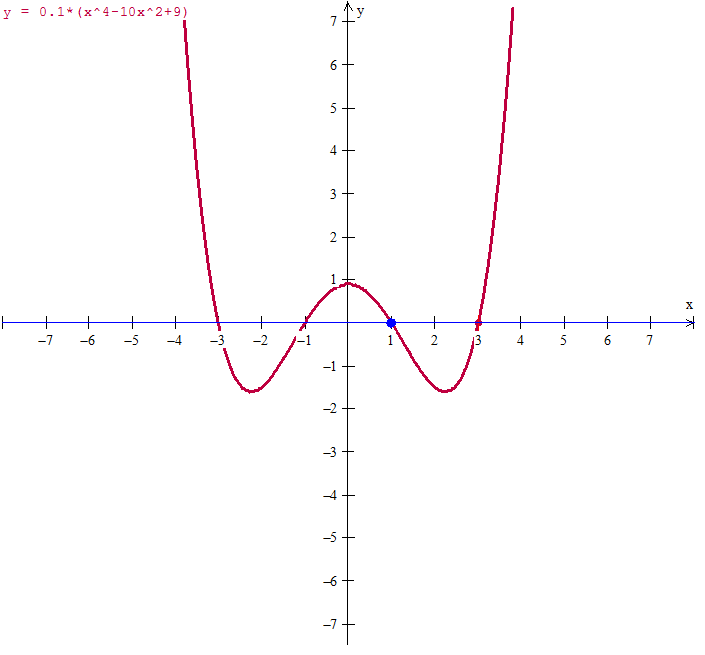
\includegraphics[width=0.4\textwidth]{horizSec}
  \caption{Secant using points $a=1$ and $b=3$, yielding the blue, horizontal line.\\ (Image created in WinPlot by Alexis Ford)}
  \label{fig:fig1}
\end{figure}

We can easily calculate (and see) that the slope of out blue secant line is $0$. If we move our points closer to $x=2$, say $a=1.5$ and $b=2.5$, we can see that the slope is closer to what we imagine our tangent line's slope should be (we can calculate the slope to be roughly $-1.69$), but we can get closer still.

\begin{figure}[h!] 
  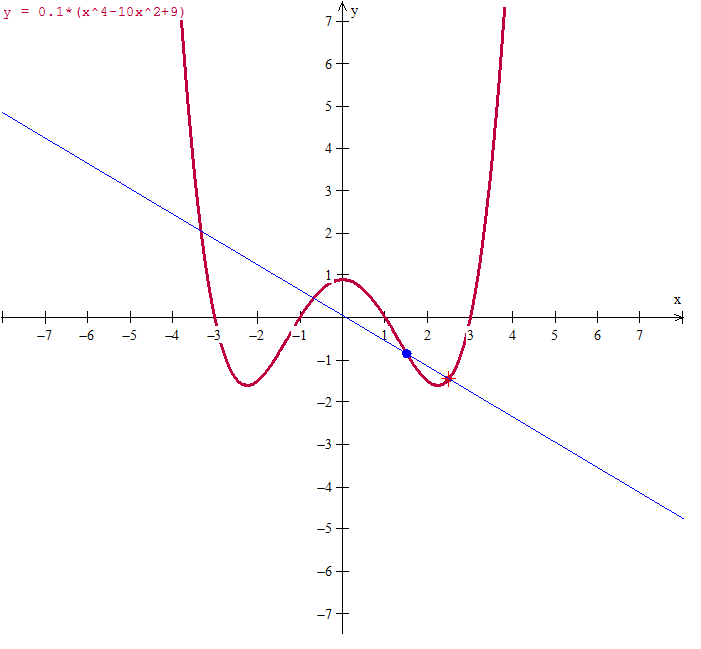
\includegraphics[width=0.4\textwidth]{closerSec} 
  \caption{Secant using points $a=1.5$ and $b=2.5$, yielding the blue line.\\ (Image created in WinPlot by Alexis Ford)}
  \label{fig:fig2}
\end{figure}

By taking the derivative, which forces our two points as close together as possible, we get our exact tangent line, $f'(2)=-\frac{4}{5}$

\begin{figure}[h!] 
  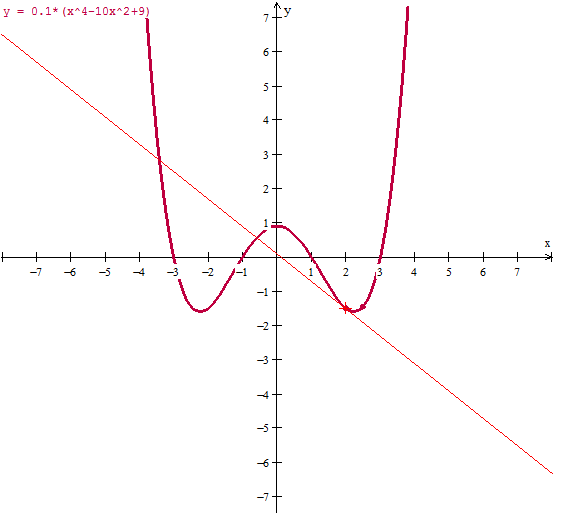
\includegraphics[width=0.4\textwidth]{tangent} 
  \caption{A red tangent line at $x=2$ with slope $f'(2)=-\frac{4}{5}$.\\ (Image created in WinPlot by Alexis Ford)}
  \label{fig:fig3}
\end{figure}
 
\section{Conclusion}
Derivatives are a powerful tool, be sure not to drink and derive.
\end{document}
